%%%%%%%%%%%%%%%%%%%%%%%%%%%%%%%%%%%%%%%%%%%%%%%%%%%%%%%%%%%%%%%%%%%%%%%%%%%%%%%%%%
\begin{frame}[fragile]\frametitle{}
\begin{center}
{\Large Introduction to Graph RAG}
\end{center}
\end{frame}

%%%%%%%%%%%%%%%%%%%%%%%%%%%%%%%%%%%%%%%%%%%%%%%%%%%%%%%%%%%
\begin{frame}[fragile]\frametitle{Challenges with LLMs}
    \begin{itemize}
        \item Learns random sentences from random people
        \item Talks like a person but doesn't really understand what it's saying
        \item Occasionally speaks absolute non sense
        \item Sensitive to question phrasing
        \item Limited to public ``knowledge''
    \end{itemize}
	
	{\tiny (Ref: The GenAI Stack - Andreas Kollegger - Neo4j)}
	
\end{frame}

%%%%%%%%%%%%%%%%%%%%%%%%%%%%%%%%%%%%%%%%%%%%%%%%%%%%%%%%%%%
\begin{frame}[fragile]\frametitle{Why Graph RAG?}
    \begin{itemize}
        \item Language models struggle with factual accuracy and real-world knowledge.
        \item Retrieval-Augmented Generation (RAG) improves accuracy using external text data.
        \item Traditional RAG has limitations in context understanding and scalability.
        \item GraphRAG leverages knowledge graphs for better retrieval and response generation.
    \end{itemize}
\end{frame}

%%%%%%%%%%%%%%%%%%%%%%%%%%%%%%%%%%%%%%%%%%%%%%%%%%%%%%%%%%%
\begin{frame}[fragile]\frametitle{Limitations of Traditional RAG}
    \begin{itemize}
        \item \textbf{Flat Retrieval:} Documents are treated as isolated entities.
        \item \textbf{Contextual Shortcomings:} Lacks deep semantic understanding.
        \item \textbf{Scalability Issues:} Slower retrieval with increasing data volume.
    \end{itemize}
\end{frame}


%%%%%%%%%%%%%%%%%%%%%%%%%%%%%%%%%%%%%%%%%%%%%%%%%%%%%%%%%%%
\begin{frame}[fragile]\frametitle{Challenges with Microsoft’s GraphRAG}
    \begin{itemize}
        \item Too expensive and impractical for large-scale industrial use.
        \item Most companies prefer standard vector databases.
        \item Lack of widespread production adoption due to cost and complexity.
    \end{itemize}
\end{frame}

%%%%%%%%%%%%%%%%%%%%%%%%%%%%%%%%%%%%%%%%%%%%%%%%%%%%%%%%%%%
\begin{frame}[fragile]\frametitle{Text-To-Cypher/SPARQL Alternative}
    \begin{itemize}
        \item Effective alternative to Microsoft’s GraphRAG.
        \item Requires costly LLM calls for query generation.
        \item Adds uncertainty due to prompt effectiveness and model performance.
        \item Increases response time and implementation complexity.
    \end{itemize}
\end{frame}

%%%%%%%%%%%%%%%%%%%%%%%%%%%%%%%%%%%%%%%%%%%%%%%%%%%%%%%%%%%
\begin{frame}[fragile]\frametitle{What is GraphRAG?}
    \begin{itemize}
        \item No universally accepted definition yet.
        \item Some associate it with Microsoft’s graph-based search approach.
        \item Others define it as querying LPG or RDF graphs using LLM-generated queries (Cypher, SPARQL).	
        \item Uses knowledge graphs instead of unstructured text.
        \item Captures entities, relationships, and hierarchical structures.
        \item Enables accurate, context-aware retrieval and response generation.
        \item Supports complex query handling with enhanced explainability.
    \end{itemize}
\end{frame}

%%%%%%%%%%%%%%%%%%%%%%%%%%%%%%%%%%%%%%%%%%%%%%%%%%%%%%%%%%%
\begin{frame}[fragile]\frametitle{Key Features of GraphRAG}
    \begin{itemize}
        \item \textbf{Structured Representation:} Uses knowledge graphs.
        \item \textbf{Contextual Retrieval:} Understands semantic relationships.
        \item \textbf{Efficient Processing:} Reduces computational cost.
        \item \textbf{Multi-Faceted Queries:} Synthesizes data from multiple sources.
        \item \textbf{Explainability:} More transparent than black-box models.
        \item \textbf{Continuous Learning:} Expands knowledge over time.
    \end{itemize}
\end{frame}

%%%%%%%%%%%%%%%%%%%%%%%%%%%%%%%%%%%%%%%%%%%%%%%%%%%%%%%%%%%
\begin{frame}[fragile]\frametitle{}

	\begin{center}
	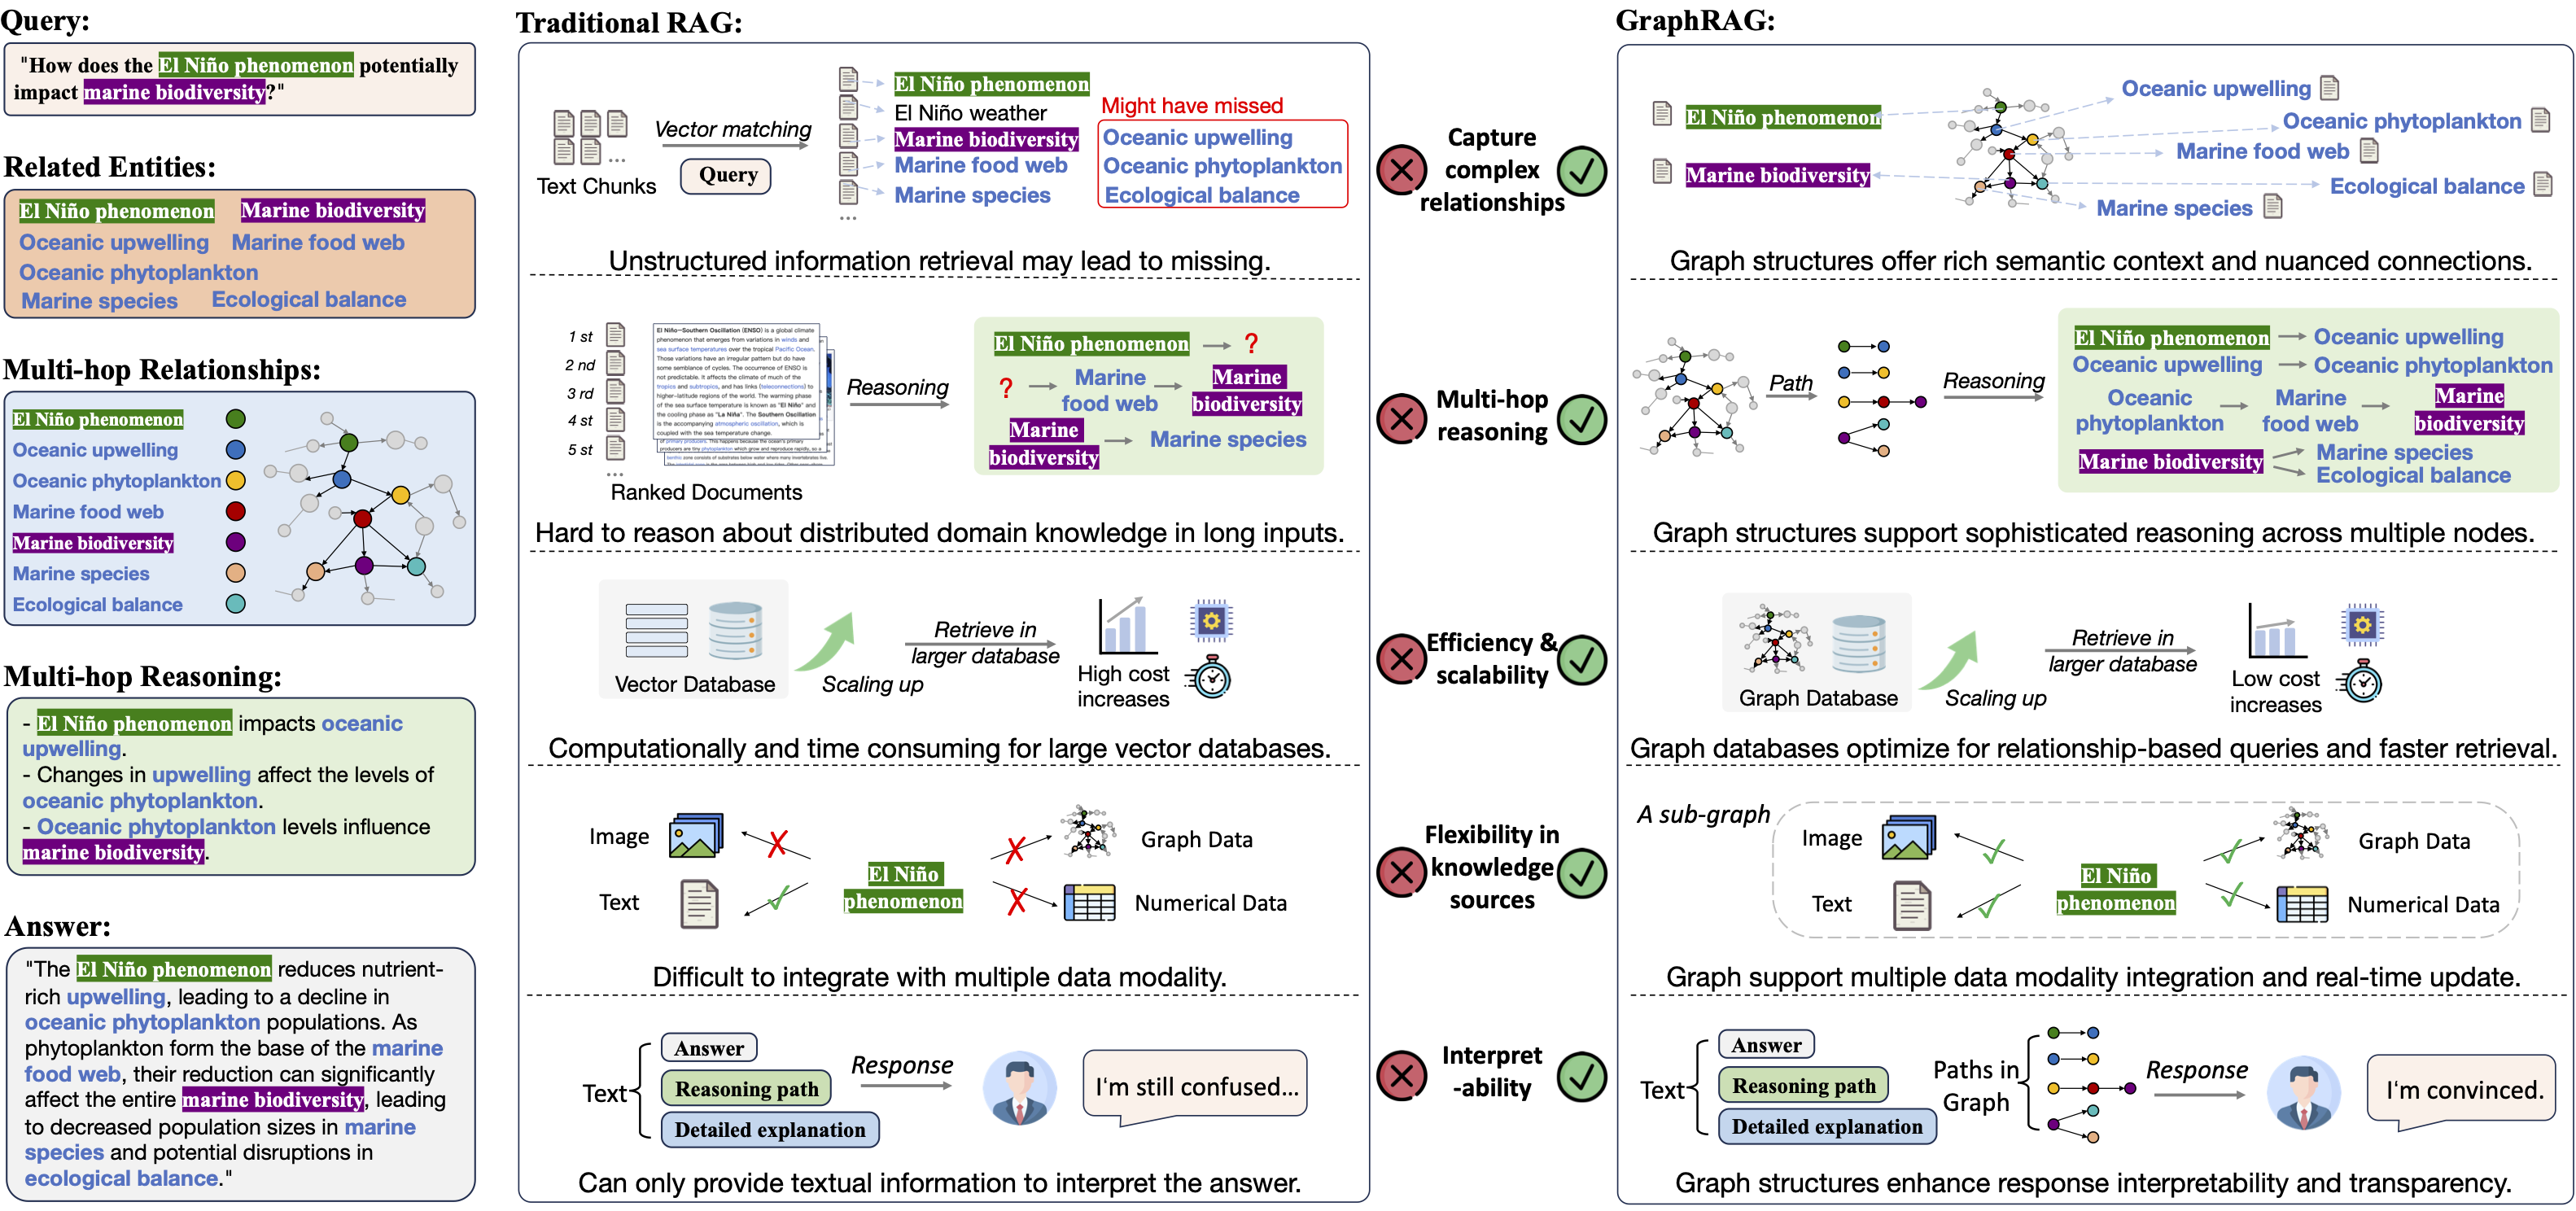
\includegraphics[width=\linewidth,keepaspectratio]{rag_vs_graphrag}
	\end{center}
	
\end{frame}


%%%%%%%%%%%%%%%%%%%%%%%%%%%%%%%%%%%%%%%%%%%%%%%%%%%%%%%%%%%
\begin{frame}[fragile]\frametitle{Applications of GraphRAG}
    \begin{itemize}
        \item \textbf{Healthcare:} Assists in diagnoses and treatment decisions.
        \item \textbf{Banking:} Detects fraudulent transactions using knowledge graphs.
        \item \textbf{Customer Service :} quickly answer customer questions from thousands of pages of policy documentation
        \item \textbf{Recommendations:} understand customer behavior and preferences better, to provide personalized services.
        \item \textbf{Supply Chain:} product recall and associated quality control checking, internal documentation search
	
    \end{itemize}

\end{frame}

%%%%%%%%%%%%%%%%%%%%%%%%%%%%%%%%%%%%%%%%%%%%%%%%%%%%%%%%%%%
\begin{frame}[fragile]\frametitle{How GraphRAG Works?}
    \begin{itemize}
        \item \textbf{Knowledge Graph Construction:} Extracts entities and relationships.
        \item \textbf{Knowledge Graph Summarization:} Generates hierarchical summaries.
        \item \textbf{Retrieval-Augmented Generation:} Uses local and global searches for queries.
    \end{itemize}
\end{frame}

%%%%%%%%%%%%%%%%%%%%%%%%%%%%%%%%%%%%%%%%%%%%%%%%%%%%%%%%%%%
\begin{frame}[fragile]\frametitle{Example of GraphRAG Representation}
    \begin{lstlisting}
    # Entities
    Type 2 Diabetes (Condition)
    High Blood Sugar Levels (Symptom)
    Nerve Damage (Complication)
    Kidney Disease (Complication)
    Cardiovascular Problems (Complication)

    # Relationships
    Type 2 Diabetes -> has_symptom -> High Blood Sugar Levels
    Type 2 Diabetes -> can_lead_to -> Nerve Damage
    Type 2 Diabetes -> can_lead_to -> Kidney Disease
    Type 2 Diabetes -> can_lead_to -> Cardiovascular Problems
    \end{lstlisting}
\end{frame}


%%%%%%%%%%%%%%%%%%%%%%%%%%%%%%%%%%%%%%%%%%%%%%%%%%%%%%%%%%%
\begin{frame}[fragile]\frametitle{Advantages of GraphRAG}
    \begin{itemize}
        \item Structured knowledge representation.
        \item Context-aware and efficient retrieval.
        \item Handles complex queries effectively.
        \item Provides explainability and transparency.
    \end{itemize}
\end{frame}

%%%%%%%%%%%%%%%%%%%%%%%%%%%%%%%%%%%%%%%%%%%%%%%%%%%%%%%%%%%
\begin{frame}[fragile]\frametitle{}

	\begin{center}
	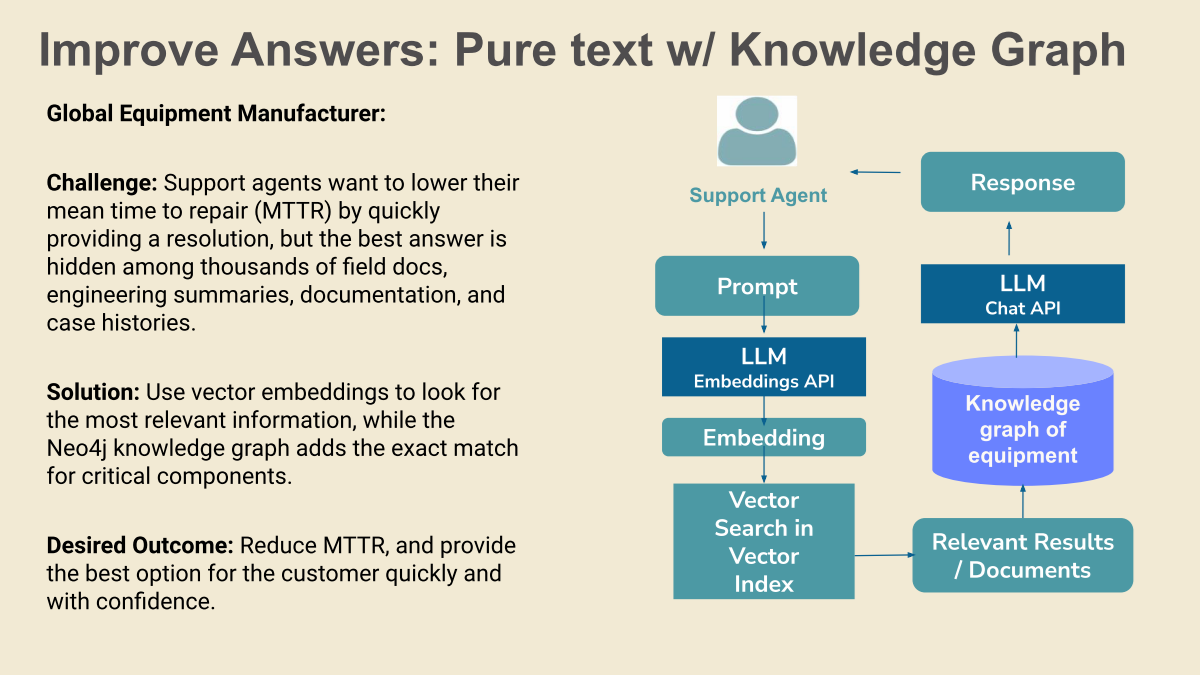
\includegraphics[width=\linewidth,keepaspectratio]{graphrag8}
	\end{center}
	
\end{frame}


%%%%%%%%%%%%%%%%%%%%%%%%%%%%%%%%%%%%%%%%%%%%%%%%%%%%%%%%%%%
\begin{frame}[fragile]\frametitle{}

	\begin{center}
	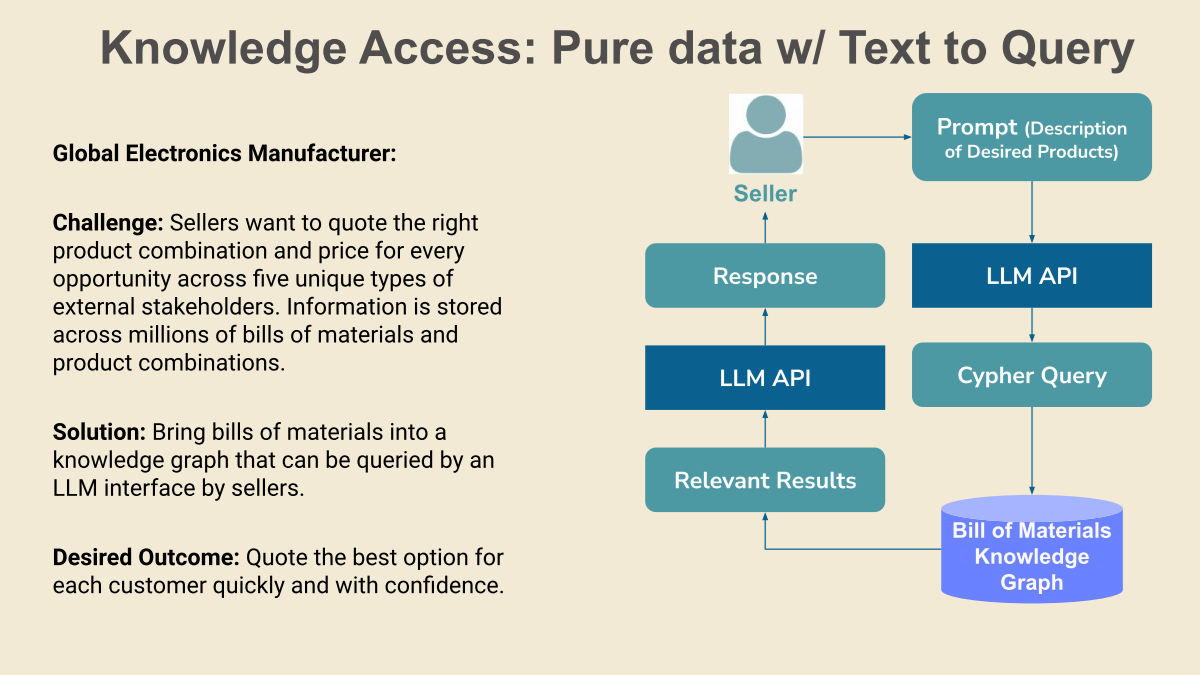
\includegraphics[width=\linewidth,keepaspectratio]{graphrag9}
	\end{center}
	
\end{frame}

%%%%%%%%%%%%%%%%%%%%%%%%%%%%%%%%%%%%%%%%%%%%%%%%%%%%%%%%%%%
\begin{frame}[fragile]\frametitle{}

	\begin{center}
	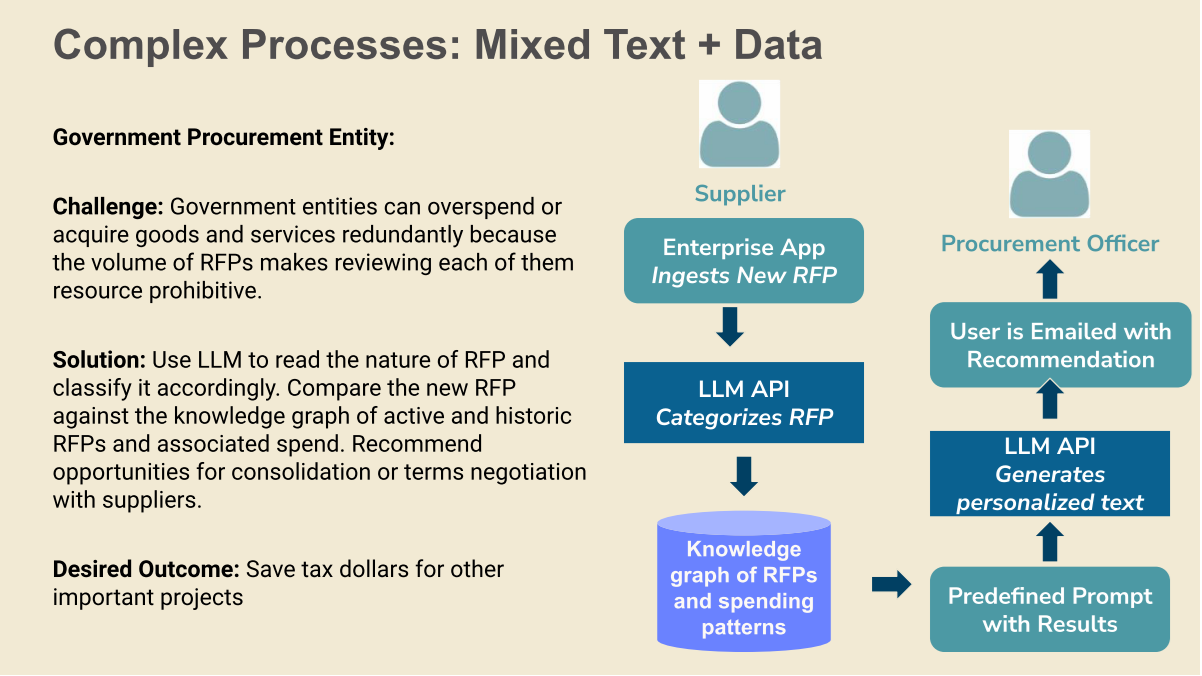
\includegraphics[width=\linewidth,keepaspectratio]{graphrag10}
	\end{center}
	
\end{frame}

%%%%%%%%%%%%%%%%%%%%%%%%%%%%%%%%%%%%%%%%%%%%%%%%%%%%%%%%%%%
\begin{frame}[fragile]\frametitle{Challenges of GraphRAG}
    \begin{itemize}
        \item \textbf{Complex Knowledge Graph Construction:} Requires sophisticated NLP techniques.
        \item \textbf{Data Dependency:} Performance relies on input data quality.
        \item \textbf{Scalability Issues:} Large graphs require significant computational resources.
    \end{itemize}
\end{frame}

%%%%%%%%%%%%%%%%%%%%%%%%%%%%%%%%%%%%%%%%%%%%%%%%%%%%%%%%%%%
\begin{frame}[fragile]\frametitle{Trend of GraphRAG Research}

	\begin{center}
	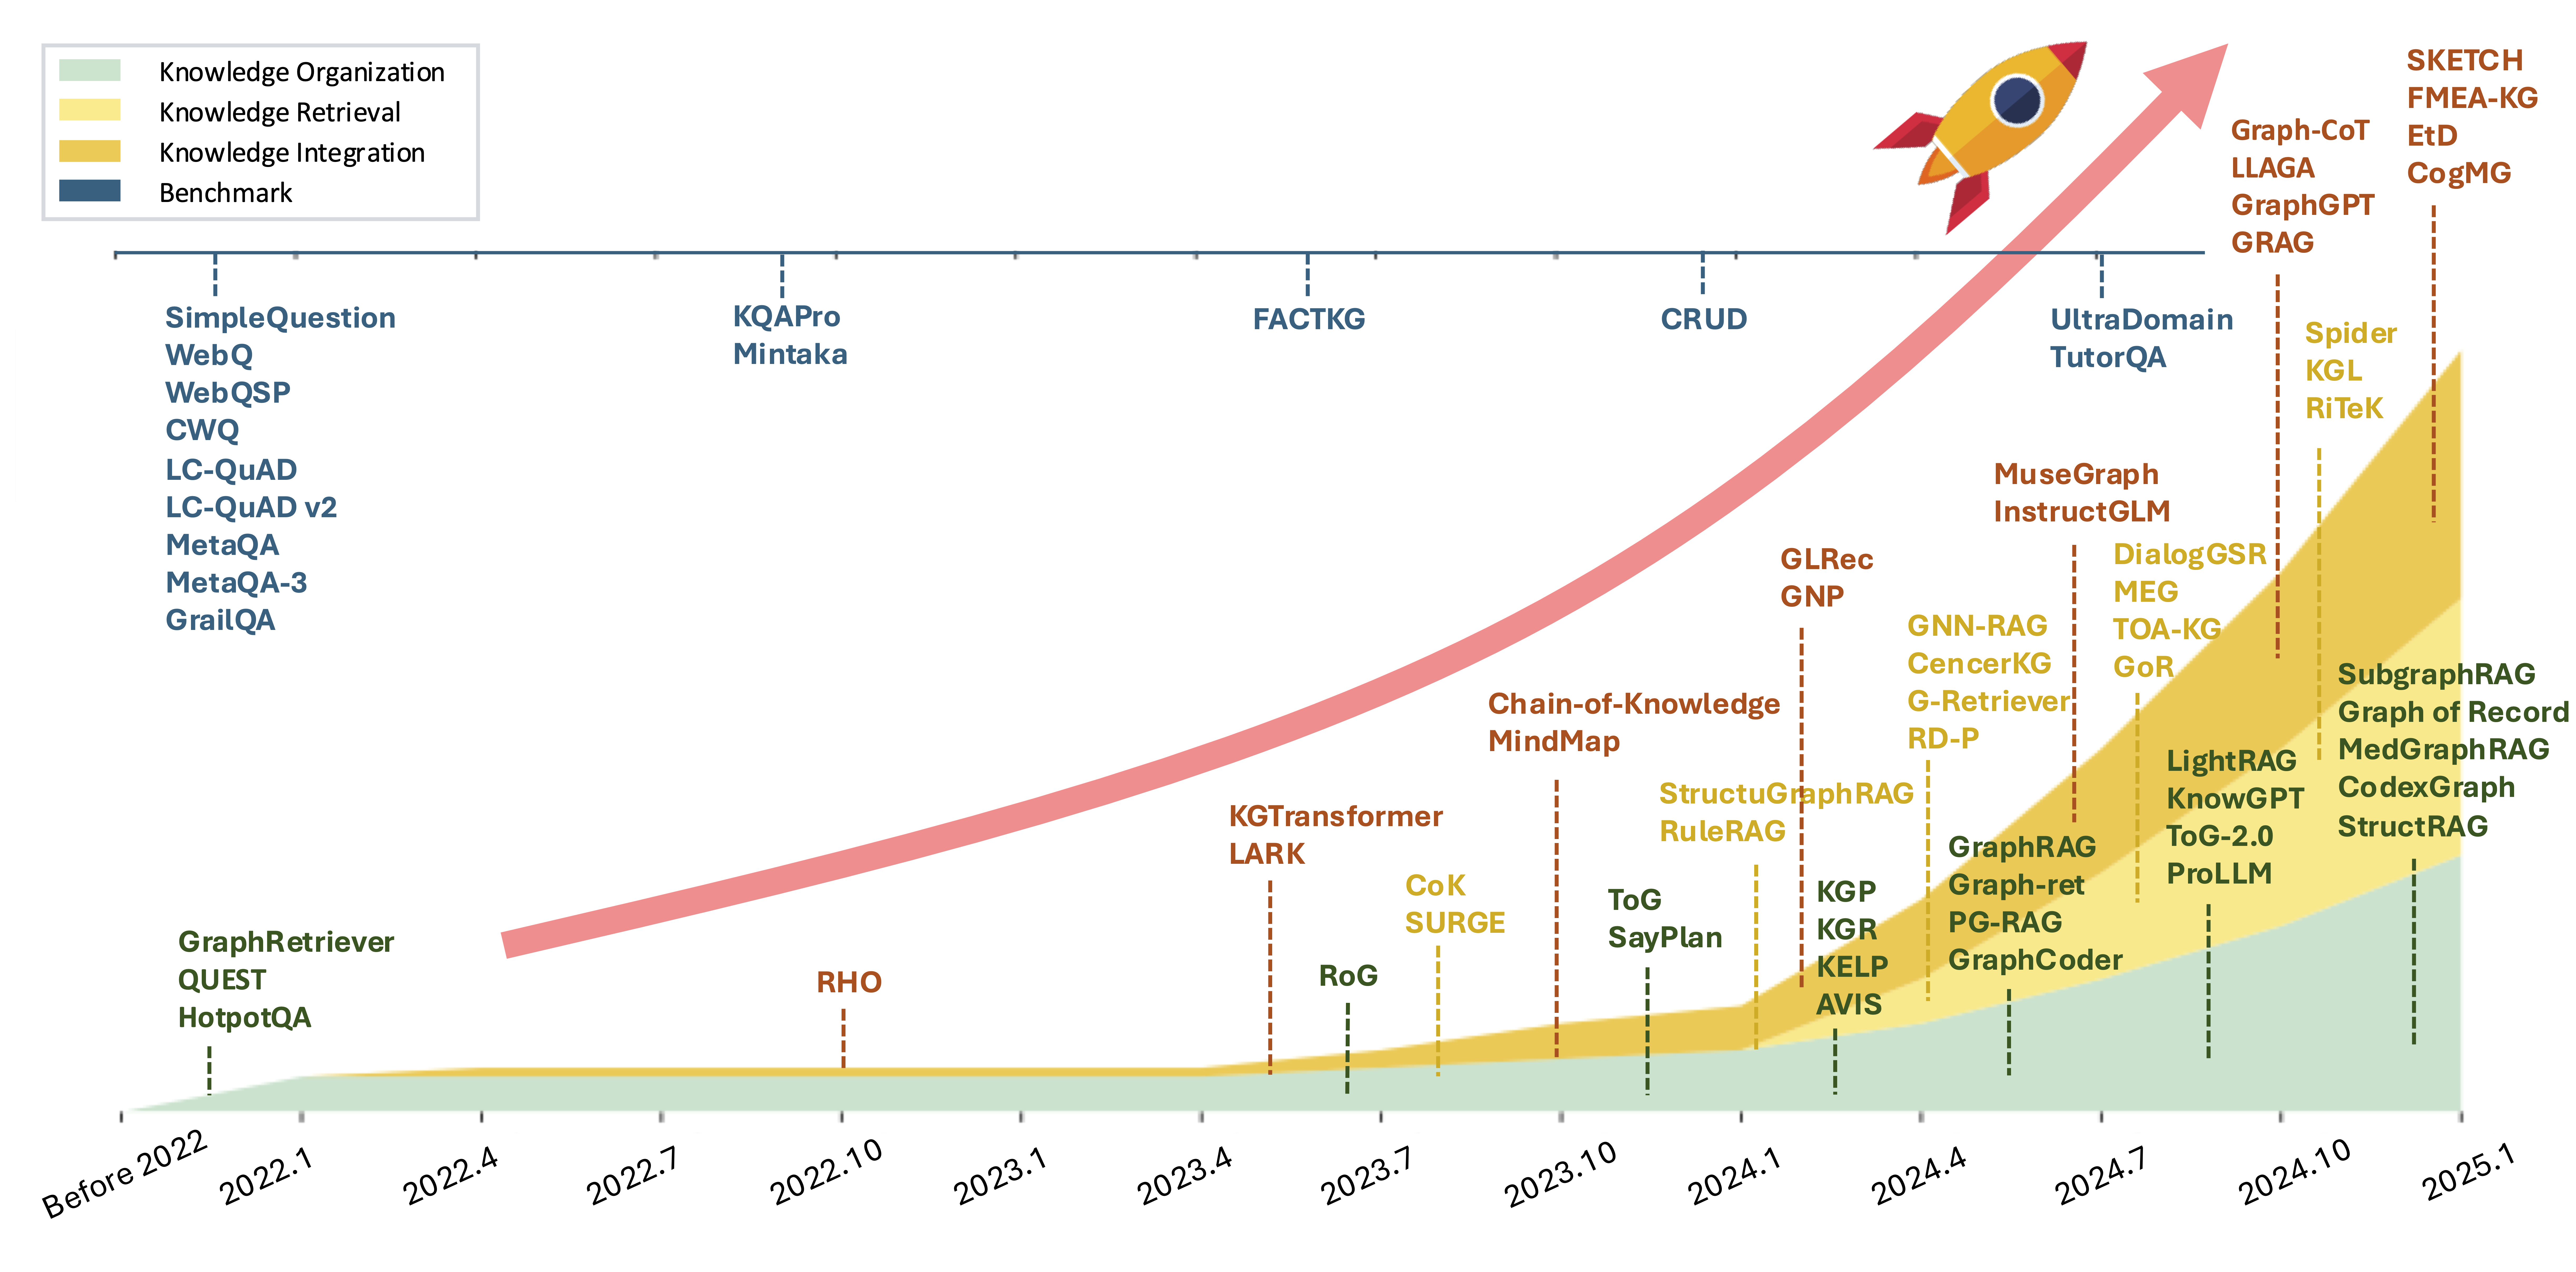
\includegraphics[width=\linewidth,keepaspectratio]{graphrag12}
	\end{center}
	
		{\tiny (Ref: Awesome-GraphRAG (GraphRAG Survey))}

	
\end{frame}

%%%%%%%%%%%%%%%%%%%%%%%%%%%%%%%%%%%%%%%%%%%%%%%%%%%%%%%%%%%
\begin{frame}[fragile]\frametitle{Conclusion}
    \begin{itemize}
        \item GraphRAG enhances traditional RAG models using structured knowledge.
        \item Improves accuracy, context-awareness, and efficiency.
        \item Useful in various domains like healthcare and banking.
        \item A promising approach for future AI-powered knowledge retrieval.
    \end{itemize}
\end{frame}
